\section{The Dataset}

The "Galaxy Zoo" dataset consists of a total \numprint{141553} images. These are split into \numprint{61578} images for training --each with their respective probability distributions for the classifications for each of the inputs-- and \numprint{79975} images for testing.

As a crowd-sourced volunteer effort, images of the dataset were classified across 11 different categories. Each of categories have attributes which volunteers can rank, there are 37 attributes in total. Some categories are dependent on the presence of others, for example number of spiral arms and spiral tightness is dependent on if the galaxy has spiral shape. The votes on these volunteer categorizations are normalized to a floating point number between 0 and 1 inclusive. A number close to 1 indicates many users identified this category for the galaxy image with a high level of confidence, while numbers close to 0 indicate otherwise. These numbers represent the overall morphology of a galaxy in 37 attributes.

Due to these probabilities being tied to each image this is a regression problem rather than a classification problem. Therefore, the task is to determine the degree to which a galaxy has certain attributes and mimic how people would classify the same galaxy.

\subsection{Decision Tree}

Morphological classification of galaxy's given by kaggle for training our model was collected by web based interface titled \href{https://www.zooniverse.org/projects/zookeeper/galaxy-zoo/classify}{Galaxy Zoo}(GZ2). User has to sign in for recording their answers. Classification process by the website are structured in a nested decision tree type. The GZ2 has 11 classification task with 37 possible responses(figure \ref{decision_tree}). The question in the starting are more general(eg, is it smooth) which move towards the specific questions(eg, how many spiral arms are there?). The appearance of subsequent questions depends upon the response of the previous question. For example, the subsequent question if the user selects smooth option as the first response will be about classifying roundness of the galaxy, which would not be shown if any other option is chosen (Figure \ref{decision_tree}).

\begin{figure}[h]
\centering
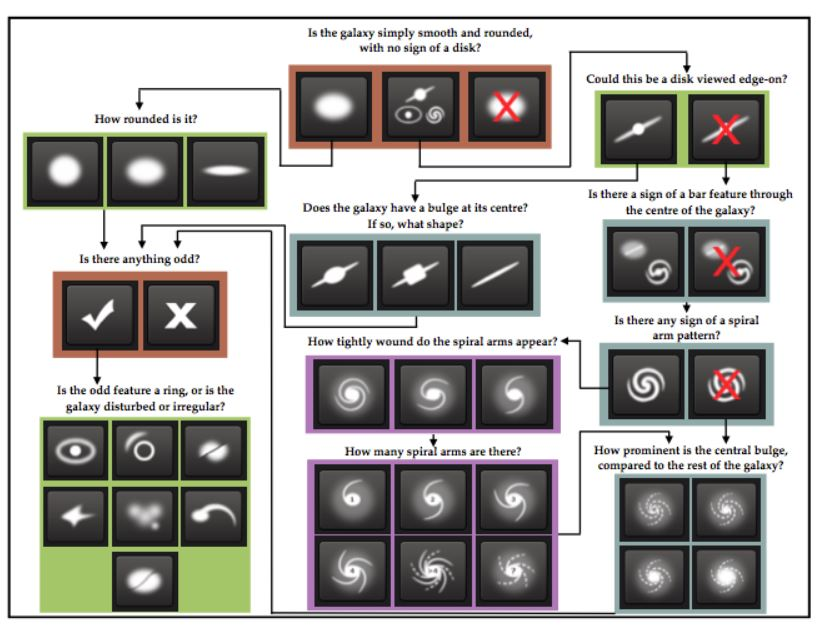
\includegraphics[scale=0.9]{figures/decision_tree.jpg}
\caption{Flowchart of the classification tasks for GZ2, beginning at the top centre. Tasks are colour-coded by their relative depths in the decision tree. Tasks outlined in brown are asked of every galaxy. Tasks outlined in green, blue, and purple are (respectively) one, two or three steps below branching points in the decision tree\cite{galaxyzoo2}.}
\label{decision_tree}
\end{figure}


As you can see in Figure \ref{decision_tree} each galaxy's classification is the result of the specific path down a decision tree. Classification performed by multiple user for the same galaxy, resulted in a multiple paths along the decision tree which generate probabilities for each node(question). In the beginning, probability of a classification will sum upto 1.0 at each node which are then weighted as following\cite{kaggledata}. Response for the first question(smooth, features/disk, star/artifact) represent the values in each category by the likelihood of the galaxy falling under that category. These values sum upto 1.0. For next questions the probabilities are first calculated (these will sum to 1.0) and then multiplied by the value which led to that new set of responses.   
